\section{Probleemi uurimine}

Ehitusfüüsika mõistes ehituskonstruktsioon kujutab endast erinevate füüsikaliste oma-dustega kihtidest 
koosnevat struktuuri, mis eraldab kaks erinevat keskkonda (näiteks: hoone sees olev õhk ja õues olev õhk).
Seejuures kõige olulisemad materjalide omadused on soojuserijuhtivus \begin{math}\lambda\end{math} [W/mK]
ja veeaurutakistus, mis võib olla väljendatud mitmel viisil (neid viise on palju, aga käesolevas töös keskendutakse 
ainult järgmistele, kuna need on kõige rohkem kasutatud nii raamatutes, kui ka materjalitootjate dokumentatsioonis):
\begin{math}\mu\end{math} - diffusioonitakistustegur (materjali omadus), Sd[m] - suhteline diffusioonitakistus 
(kindla paksusega toote omadus). 

\begin{figure}[ht]
    \centering
    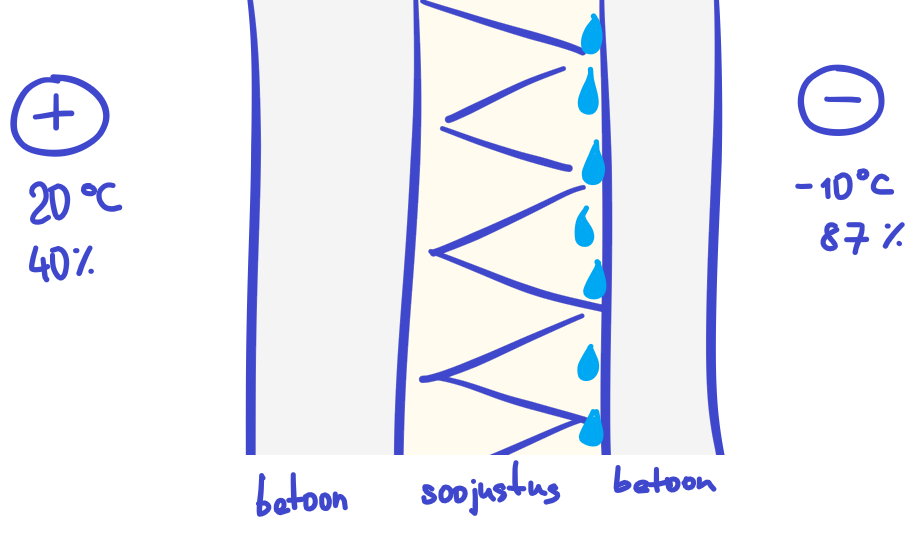
\includegraphics[width=.6\textwidth]{figures/problem_statement/07_layered_structure_sample.png}
    \caption{\textit{Kihilise konstruktsiooni näide}}
    \label{fig:construction_sample}
\end{figure}

Teatud tingimustel võib tekkida olukord, kui konstruktsiooni sees on mingis punktis suhteline niiskus
nii kõrge, et soodustab bioloogiliste kahjustuste või isegi kondensaadi tekkimist. Nimetatud olukord on ohtlik
nii ehituskonstruktsioonile, mis pikaajalise niiskuse mõjul lagunevad, kui ka inimese tervisele, sest konstruktsioonide
sees olev hallitus on õhku sattuvate bakterite allikaks. Seda, kuidas konstruktsioon töötab soojus- ja niiskuse leviku
seisukohalt nimetatakse konstruktsiooni niiskustehniliseks toimivuseks. Arvutust, mille eesmärgiks on hinnata 
kondenseerumise riski konstruktsioonis, nimetatakse konstruktsiooni niiskustehnilise toimivuse analüüsiks.

Tegemist on klassikalise ehitusfüüsika ülesandega, mille lehandemiseks peab ette võtma järgmiseid samme:
\begin{itemize}
    \item konstruktsiooni kihtide soojustakistuse ja konstruktsiooni summaarse soojustakistuse arvtus
    \item temperatuuri jaotuse määramine kihtides sõltuvalt sise- ja väliskeskkonna temperatuuridest ning 
    soojustakistuste väärtustest
    \item konstruktsiooni kihtide veeaurutakistuse ja konstruktsiooni summaarse veeaurutakistuse arvutus
    \item veeauru küllastusrõhu jaotuse määramine lähtuvalt temperatuuri jaotusest
    \item veeauru osarõhu jaotuse määramine kihides sõltuvalt sise- ja väliskeskkonna parameetritest ning 
    veeaurutakistuse väärtustest
    \item tulemuste esitamine graafiliselt diagrammil
    \item arvutuste kordamine erinevate sise- ja väliskeskkonna parameetrite kombinatsioonidega
\end{itemize}

Ülesande käsitsi lahendades, koostatakse tabelit, mille ridadesse pannakse kirja kihid ja veergudesse arvutatakse 
väärtused. Kuigi arvutused ise ei ole väga keerulised (tegemist on tavaliste füüsika valemitega), paraku käsitsi arvutamine 
võtab tohutult palju aega. Microsoft Excel võimaldab teatud määral protessi automatiseerida, kuid siiski mõned 
tegevused (näiteks uute kihtide lisamine, või kihtide järjekorra muutmine) jäävad suures osas käsitööks, mis võtab palju 
aega ja ka soodustab vea tegemist. Pildil \ref{fig:excel_table_sample} on toodud sellise tabeli näide.
\begin{figure}[ht]
    \centering
    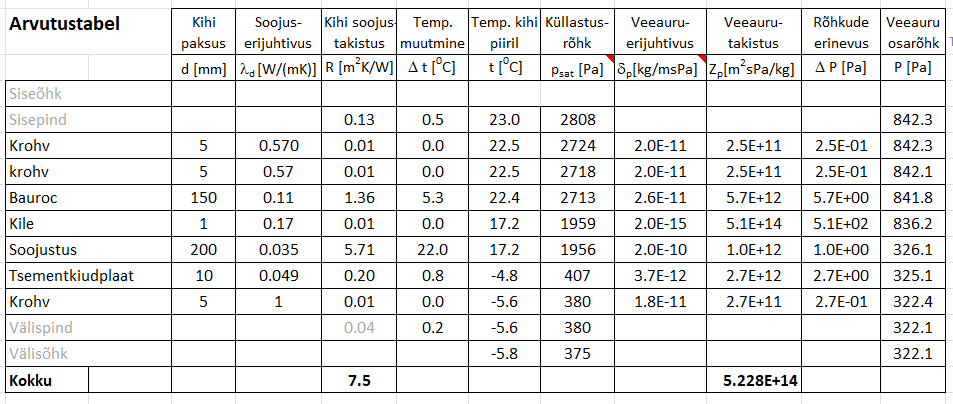
\includegraphics[width=.8\textwidth]{figures/problem_statement/04_calc_table.png}
    \caption{\textit{Arvutustabeli näide}}
    \label{fig:excel_table_sample}
\end{figure}

Analüüsi tulemused esitatakse graafiliselt diagrammi kujul, mille \begin{math}x\end{math} telg on 
punkti asukoht konstruktsioonis ning \begin{math}y\end{math} teljel on temperatuuri, veeauru küllastus- ja
osarõhu väärtused vastavas punktis -- näide on todud pildil  \ref{fig:excel_graph_sample}.

\begin{figure}[ht]
    \centering
    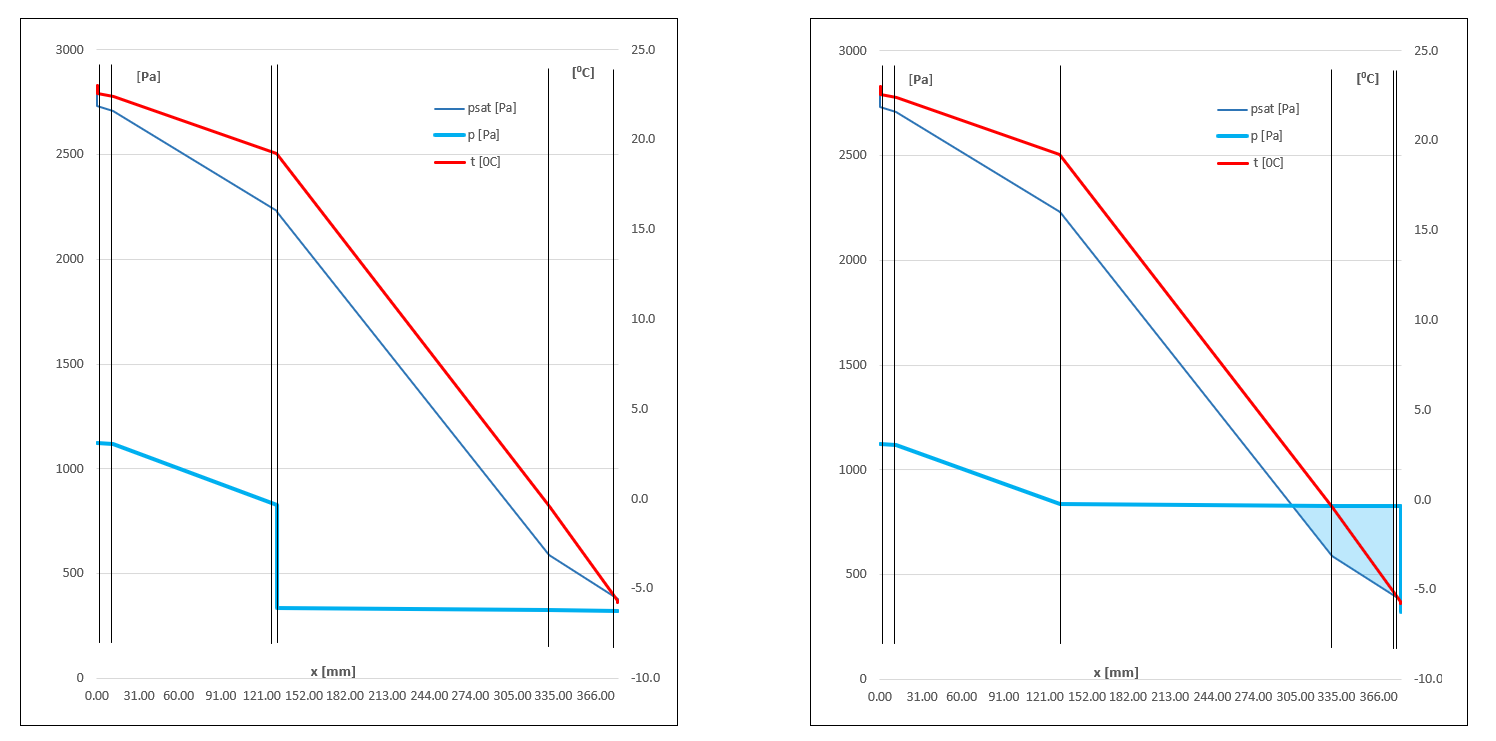
\includegraphics[width=.8\textwidth]{figures/problem_statement/05_excel_grafic_sample.png}
    \caption{\textit{Näide tulemuste esitamisest graafikul}}
    \label{fig:excel_graph_sample}
\end{figure}

Graafik annab väga head visuaalset ülevaadet konstruktsiooni kihtides toimuvale. Täpsemalt öeldes peab vaatama 
veeauru küllastus- ja osarõhkude jaotuste graafikuid. Veeauru osa- ja küllastusrõhu suhe on suhteline niiskus. 
Mida lähedam osarõhu graafiku joon küllastusrõhu graafiku joonele, seda kõrgem on suhteline niiskus. Punkt, milles
need jooned ristuvad on suhteline niiskus 100\%, mis tähendab kondensaadi tekkimist --  sellist punkti nimetatakse kastepunktiks.
Näide on toodud pildil \ref{fig:excel_graph_sample}: vasakul on niiskustehniline olukord hea, kuna aurutõke asub õiges kohas, ning paremal
paiknem konstruktsiooni külmemal pool veeaurupidav kiht, mistõttu läheb osarõhk kõrgeks ja ületab küllastusrõhu väärtust.


Kuigi probleem on üldiselt lahendatav näiteks \textit{Microsoft Excel} vahenditega, paraku pole see kõige mugavam viis
mitmel põhjustel:
\begin{itemize}
    \item selline lähenemine vajab palju käsitööd kihtide lisamiseks või ümber paigutamiseks, mis on analüüsi lahutamata osa -- proovitakse erinevaid materjale erinevates konstruktsiooni kohtades
    \item materjalide omadusi omadusi on siiski vaja leida ja TODO !
\end{itemize}


Kohalikul turul puudub tarkvara, millega oleks mugav teostada konstruktsiooni
niiskustehnilise toimivuse analüüsi. Niiskustenilise toimivuse analüüs on klassikaline ehitusfüüsika ülesanne, mille 
eesmärk on hinnata veeauru kondenseerumise (või ka kõrgest niiskusest põhjustatud kahjustuste tekkimise) riski.




\section{Olemasolevad lahendused ja turu analüüs}
Üks populaarsematest analoogidest, mida kasutatakse sealhulgas ka Eestis, on Saksa päritoluga tarkvara \textbf{Ubakus}. 
Tegemist on veebirakenduse kujul kommertstarkvaraga, mille \textit{demo}-versioon on saadaval tasuta (pilt \ref{fig:ubakus_sample}). 
\begin{figure}[ht]
    \centering
    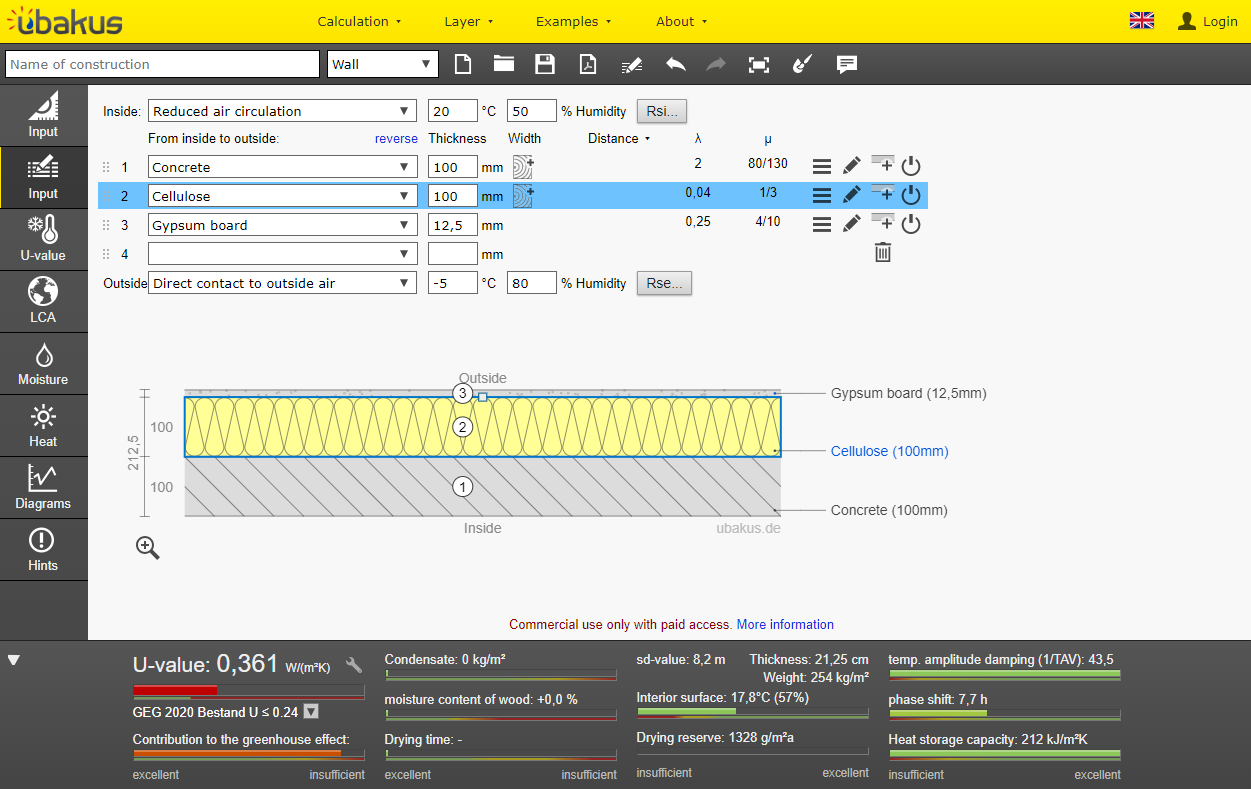
\includegraphics[width=.8\textwidth]{figures/problem_statement/01_ubakus.png}
    \caption{\textit{Ubakus veebirakenduse ekraanitõmmis.}}
    \label{fig:ubakus_sample}
\end{figure}

\textbf{Ubakus} võimaldab teostada konstruktsiooni niiskustehnilist analüüsi. Kasutajaliides võidaldab 
mudeldada mitmest kihist koosneva konstruktsiooni, valides igale kihile paksust ja materjali, millest 
kiht koosneb. Tugev eelis on see, et tarkvaraga saab analüüsida ka mittehomogeensete (mitemest erinevast 
materjalist, nt puitsõrestiksein) kihtidega konstruktsioone - pilt \ref{fig:ubakus_layers}

\begin{figure}[ht]
    \centering
    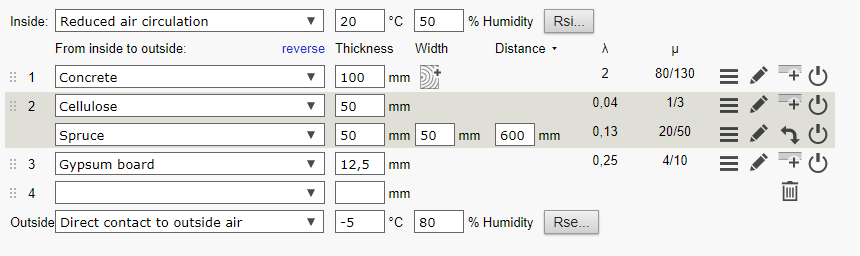
\includegraphics[width=.6\textwidth]{figures/problem_statement/02_ubakus_layers.png}
    \caption{\textit{Ubakus: konstruktsiooni kihtide lisamine.}}
    \label{fig:ubakus_layers}
\end{figure}

Ehitusmaterjalide valik, mida on võimalik konstruktsiooni mudeldamisel kasutada, on piisavalt lai 
(aga tasuta versioonis piiratud). Tasulises versioonis on samuti võimalik ka oma materjalide 
lisamine ja kasutamine. Puuduseks on see, et teatud osa baasis olevatest ehitusmaterjalidest on Saksamaal
turustatavad materjalid, mistõttu selle tarkvara kasutades Eestis peab kas sisestama kõik vajalikud 
materjalid käsitsi, või kasutada Saksa analoogid ning arvestada sellest tulenevaarvutuste ebatäpsusega.
\begin{figure}[ht]
    \centering
    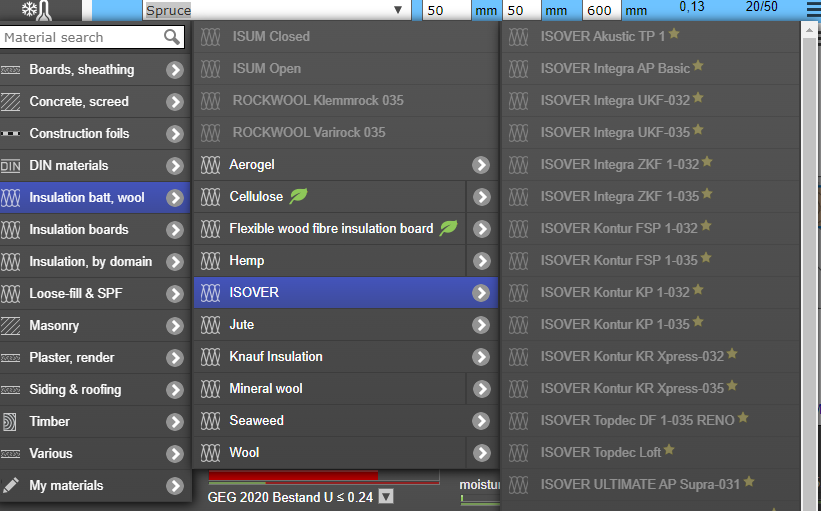
\includegraphics[width=.6\textwidth]{figures/problem_statement/03_ubakus_materials.png}
    \caption{\textit{Ubakus: ehitusmaterjalide valik baasis.}}
    \label{fig:ubakus_materials}
\end{figure}
